\documentclass[12pt]{article}
% Packages and macros
\usepackage[T1]{fontenc}
\usepackage{mathptmx}
\usepackage{pgf}
\usepackage{pgfpages}
\usepackage{parallel}
\usepackage{siunitx}
\usepackage{booktabs}
\usepackage{fancyhdr}
\usepackage{datetime}
%\usepackage[utf8]{inputenc}
\usepackage{graphicx}
\usepackage{blindtext}
\usepackage{multicol}
\usepackage{enumerate}
\usepackage{pifont}
\usepackage{amssymb}
\usepackage[export]{adjustbox}
\usepackage[margin=1in]{geometry}
\usepackage[francais]{babel}
\usepackage{caption}
\newcommand{\source}[1]{\vspace{-12pt} \caption*{Source: {#1}} }
\usepackage{amsmath}
\usepackage{xcolor}
\usepackage{array}
\usepackage{tabularx}
\usepackage[thinlines]{easytable}

\newdateformat{monthyeardate}{%
  \monthname[\THEMONTH], \THEYEAR}

\pgfpagesdeclarelayout{boxed}
{
  \edef\pgfpageoptionborder{0pt}
}
{
  \pgfpagesphysicalpageoptions
  {%
    logical pages=1,%
  }
  \pgfpageslogicalpageoptions{1}
  {
    border code=\pgfsetlinewidth{1pt}\pgfstroke,%
    border shrink=\pgfpageoptionborder,%
    resized width=.98\pgfphysicalwidth,%
    resized height=.98\pgfphysicalheight,%
    center=\pgfpoint{.5\pgfphysicalwidth}{.5\pgfphysicalheight}%
  }%
}
\pgfpagesuselayout{boxed}
\setlength{\columnsep}{0.5cm}

% \renewcommand\thesubsection{\Alph{subsection}}

\begin{document}
\pagestyle{fancy}
\lhead{EIND}
\chead {\today}
\rhead{TP0}
\fontsize{16}{16}\selectfont

% ------------------------- TITLE PAGE INSERTION ------------------------ 
\begin{titlepage}
   \begin{center}
        \vspace*{1cm}
        \LARGE
        \textbf{Industrial Electronics \\ Practicum 0}
        
        \vspace{0.3cm}
        Summary on linear regulator LM317
            
        \vspace{1.5cm}

        \textbf{Miguel Santos \\ Ali Zoubir}

        \vfill
            
        Laboratory report
            
        \vspace{0.8cm}
     
        
\includegraphics[width=0.31\textwidth]{ETML-ES-LOGO.png}

        Electrical engineering\\
        Superior school\\
        Switzerland\\
        \monthyeardate\today
            
   \end{center}
\end{titlepage}
\clearpage

% -------------------------- ABSTRACT ----------------------------------- 
\section*{Abstract}
{
During this practicum we had to learn, design, implement, simulate, measure, and analyze a linear regulator model using the LM317 IC.\\ 
This practicum motivates the student to understand linear regulation systems, how to size it, and be critical of its characteristics.\\
Our observations in the report shows that  ........
}
\clearpage

% --------------------- TABLE OF CONTENTS  ------------------------------- 
\tableofcontents
\clearpage

% ------------------------- INTRODUCTION --------------------------------- 
\section{Introduction}
This practicum aims to study, dimension, simulate, and implement an LM317 linear regulator system, and analyze different aspects and parameters that impact the circuit's functionality. \vspace{+12pt}

The LM317 is a voltage regulator that is commonly used in electronic circuits. It is designed to provide a constant output voltage, regardless of variations in input voltage or load. It does this by using a reference voltage and an adjustable resistor to control the output voltage. The reference voltage is set using a pair of external resistors, and the output voltage can be adjusted by changing the resistance of the adjustable resistor. This allows the LM317 to be used in a wide range of applications, such as providing a stable power supply for a circuit or controlling the output voltage of a battery.
\clearpage


% ------------------- PRELIMINARY TASK (TASK0) --------------------------- 
% ------------------------- PRELIMINARY TASK -----------------------------
\section{Preliminary task}
Our goal is to implement an LM317 regulation system, which has an input of \textbf{5V} and an output of \textbf{3V3}. To accomplish that, we must scale different parameters, that we will develop in the subsection \ref{ssec:num01} to \ref{ssec:num05}

% ---------------- Subsection 1 ----------------
\subsection{Resistive bridge sizing} \label{ssec:num01}
{
\begin{figure}[!htb]
    \centering
    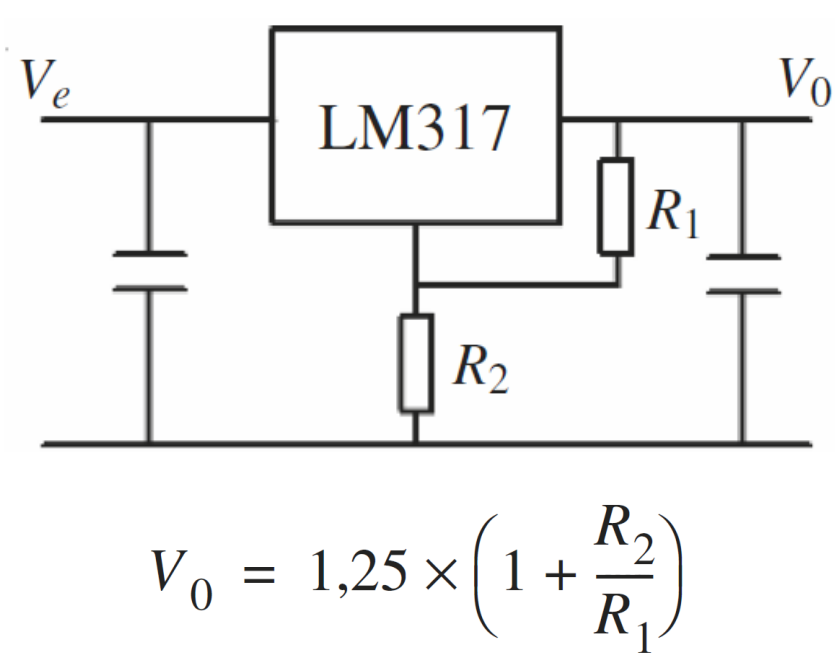
\includegraphics[width=50mm]{../Figures/LM317-Schematic.PNG}
    \caption{Resistive-bridge schematic and formula in the datasheet}
    \source{LM317 datasheet}
    \label{fig:Rbridge}
\end{figure}

The formula in the datasheet neglects the breakdown current of the internal Zener diode, we decided to take consideration of it in our calculations.

\begin{figure}[!htb]
    \centering
    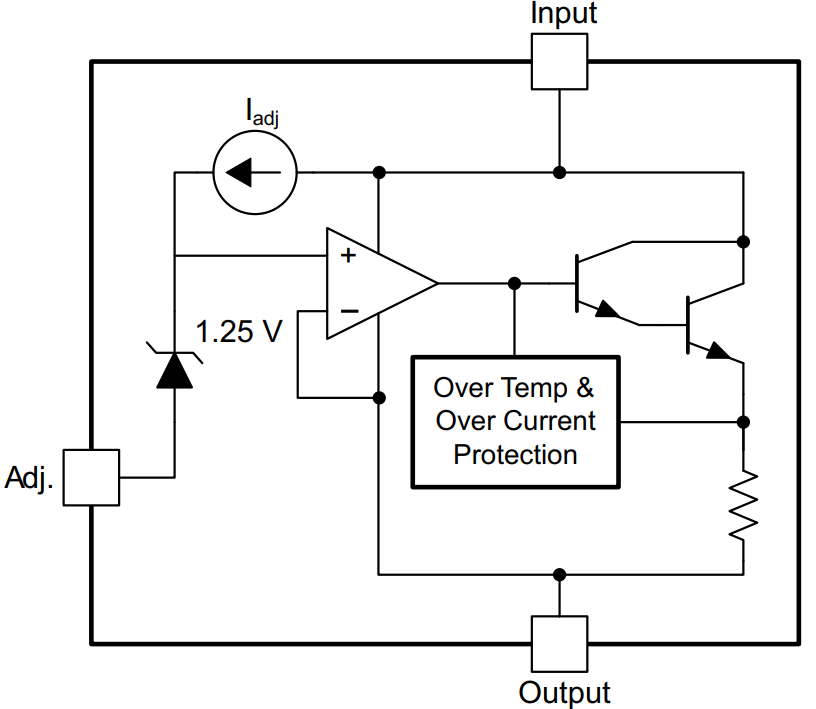
\includegraphics[width=45mm]{../Figures/Inside-LM317.PNG}
    \caption{Functional bloc diagram of LM317}
    \source{LM317 datasheet}
    \label{fig:FuncLM317}
\end{figure}

The voltage of the internal zener diode is \textbf{1.25V}, this is the reference and minimum voltage of the regulator. To dimension the resistive bridge, we must take into account the breakdown current of the diode which is \textbf{50uA}, when this condition is met, we know that the voltage between the output and the ADJ pin is the same as the reference voltage. We can then set an arbitrary value for one of the resistors knowing that the total voltage at the output must be \textbf{3.3V}. We decided to have a current of \textbf{50uA} through R1, to reduce the power dissipation in the bridge.

\clearpage

\subsubsection{Sizing formulas}
{
As described bellow, we have as parameters:\\
$ I_{adj} = 50 [uA] $ \\
$ I1 = 50 [uA] $ \\
Where I1 has been fixed by us to avoid having too much unnecessary current in the resistor bridge..\\
$ U1 = 1.25 [V] $ 

\begin{equation} \label{equ_R1}
     R1 = \frac{U1}{I1} \\
\end{equation} 
\begin{equation} \label{equ_R2}
     R2 = \frac{U2}{I2} = \frac{Uout - U1}{I_{adj}+I1} 
\end{equation}  
As equation (\ref{equ_R1}) and (\ref{equ_R2}) state, in our application we found the values: 
\\ {$ R1 = 25 \ k\Omega $ \\ $ R2 = 20.5 \ k\Omega $}
}

}

% ----------------Subsection 2 ----------------
\subsection{Maximum output power calculation} \label{ssec:num02}
{
Since we have very few loss current in the resistive bridge, we decided to neglect it. \\
We have as parameters: \\
$ U_{in} = 5 [V] $ \\
$ U_{out} = 3.3 [V] $ \\
$ I_{out} = 100 [mA] $ (Specification) \\
\begin{equation} \label{equ_Pmax}
     P_{max} = (U_{out}-U_{in})*I_{out} \\
\end{equation} 
By applying equation number (\ref{equ_Pmax}) to our application, we found the value: \\ 
{$ P_{max} = 330 \ mW $}

}

% ----------------Subsection 3 ----------------
\subsection{Input provided power} \label{ssec:num03}
{
In this subsection, we will continue to neglect the diode breakdown current. To have as an output current \textbf{100 mA} we sized an output resitor by applying this formula:
\begin{equation}
    R_L = \frac{U_{out}}{I_{out}}
\end{equation}
So our load resistor value is $ \mathbf{ 33 \ \boldsymbol{\Omega} } $. \\
\clearpage
We can now define our different powers in the systems:

\begin{equation}
    P_{out} = U_{out}*I_{out}
\end{equation}

\begin{equation}
    P_{in} = U_{in}*I_{out}
\end{equation}

\begin{equation}
    P_{reg} = P_{in} - P_{out}
\end{equation}
Calculated values for our application:\\
$ P_{out} = 330 \ mW $ \\
$ P_{in}  = 500 \ mW $ \\
$ P_{reg} = 170 \ mW $ \\
}

% ----------------Subsection 5 ----------------
\subsection{Temperature of the LM317 junction without cooling} \label{ssec:num05}
{
Finally, we have been asked to estimate the temperature of the LM317 junction, without cooling. Specification set the ambient. The datasheet provides us the thermal resistance between the junction and the ambient. So we have : \\
$ T_{A} = 35 \ °C $ \\
$ Rth_{JA} = 37.9 °C/W $\\
We can define the temperature of the junction by :
\begin{equation*}
	T_{J} = T_{A} + Rth_{JA} * P_{reg}
\end{equation*}

Calculated value for our application:\\
$ T_{J} = 41,44 \ °C $ \\

}

\newpage

\subsection{Simulation of the system} \label{ssecNum06}
{
In this section we will simulate our system to corroborate our previously dimensioned system (From section \ref{ssec:num01} to \ref{ssec:num03}).	
	
\underline{Simulation schematic :} \\

\begin{figure}[h]
	\centering
	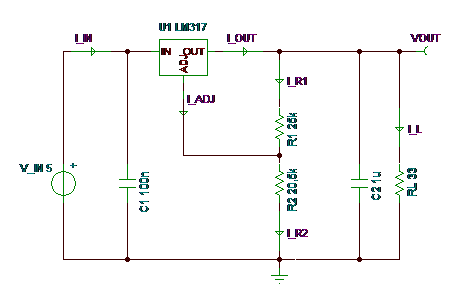
\includegraphics[width=0.53\linewidth]{../../Simulations/premiere_partie/pont_diviseur}
	\caption{Schematic of the first part}
	\label{fig:pontdiviseur}
	\source{Authors}
\end{figure}
	
\underline{Simulation method :}\\
In order to perform our simulations, we used the DC analysis tool of Tina TI.

\underline{Simulation results and analysis :}\\
\begin{figure}[h]
	\centering
	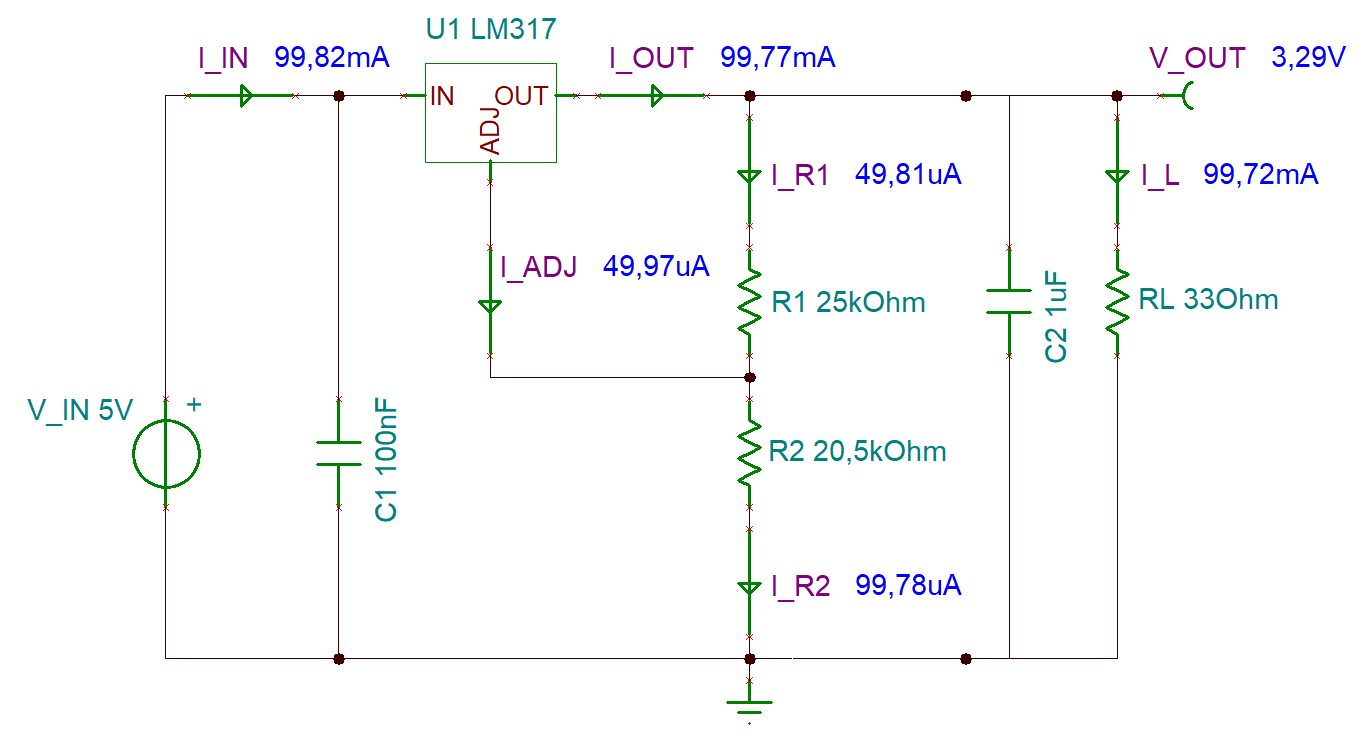
\includegraphics[width=0.53\linewidth]{../../Simulations/premiere_partie/tension_3v3}
	\caption{Simulation of the first task}
	\label{fig:tension3v3}
	\source{Authors}
\end{figure}


As we can see on the figure \ref{fig:tension3v3}, the output voltage is well dimensioned knowing that there is \textbf{3.3V} on the load resistance, and a current of \textbf{100mA}. We can also see that the breakdown current of the diode is $ \sim 50 \mu A $ which is consistent with the datasheet.

}

\clearpage

% ------------------------ MAIN TASK (TASK1) ----------------------------- 
% ------------------------- MAIN TASK ---------------------------------
\section{Main task}
\subsection{Schematic proposal for limiting output current to 250mA} \label{ssec:num11}
{
	We were asked to design a proposed scheme to limit the output current to 250mA, to do this we decided to change the principle of the connections to create a current source using the LM317.
	
	
	A
	
}

\subsection{Plotting output tension depending on output current} \label{ssec:num12}
{}
\subsection{Oscillogram of the output current depending on the input tension} \label{ssec:num13}
{}
\subsection{Dissipated power calculation} \label{ssec:num14}
{}
\subsection{Estimation of the junction's temperature without cooling} \label{ssec:num15}
{}
\subsection{Short-circuited output - dissipated power calculation} \label{ssec:num16}
{}
\clearpage

\end{document}
